
%----------extends build------------ 
\chapter{  Extendbuild : Ajout des composants avancés}
\minitoc
\clearpage

\section{Introduction}
L’enrichissement du système minimal s’articule autour de deux axes :

\begin{itemize}
 
  \item Installation d’outils et de paquets complémentaires (sécurité, gestion de fichiers et de disques, éditeurs de texte, réseau, etc.).
  \item Configuration de l’environnement graphique ;  
\end{itemize}

\section{Sécurité}
La sécurité se décline en trois volets : l’accès, la prévention et la détection.

\begin{enumerate}
  \item \textbf{Accès} : gestion des sessions utilisateur via l’authentification (login) et renforcement des politiques d’accès à l’aide de modules PAM. Protection de l’accès réseau par des règles iptables (pare‑feu).
  \item \textbf{Prévention} : lutte contre les maliciels (trojans) et chiffrement des données, notamment avec GnuPG.
  \item \textbf{Détection} : surveillance des altérations de fichiers critiques grâce à des outils enregistrant des « empreintes » (hashes).
\end{enumerate}

Exemple des Outils de sécurité installés:
\begin{table}[H]
    \centering
    \begin{tabular}{|c|p{8cm}|}
        \hline
        \textbf{Paquet}  & \textbf{Fonction principale} \\
        \hline
       
        CrackLib  & Vérification de la robustesse des mots de passe contre les attaques par dictionnaire. \\
        \hline
        iptables  & Configuration du pare-feu natif du noyau Linux via des règles de filtrage. \\
        \hline
        GnuPG  & Chiffrement/déchiffrement de données et signatures numériques (implémentation OpenPGP). \\
        \hline
        Sudo  & Délégation sécurisée de commandes privilégiées aux utilisateurs autorisés. \\
        \hline
        Linux-PAM & Framework modulaire pour l'authentification système (login, mot de passe, etc.). \\
        \hline
        OpenSSH  & Suite d'outils de connexion sécurisée à distance . \\
        \hline
        Polkit  & Contrôle granulaire des privilèges pour les processus non-root. \\
        \hline
        Shadow  & Gestion sécurisée des comptes utilisateurs et des mots de passe chiffrés. \\
        \hline
    \end{tabular}
    \caption{Paquets critiques pour la sécurité système}
    \label{tab:security_packages}
\end{table}
 
%\begin{table}[H]
%    \centering
%    \begin{tabular}{|c|c|p{8cm}|}
%        \hline
%        \textbf{Paquet} & \textbf{Version} & \textbf{Fonction principale} \\
%        \hline
%        make-ca & 1.14 & Gestion des certificats racines TLS et mise à jour des magasins de confiance système. \\
 %       \hline
 %       CrackLib & 2.10.2 & Vérification de la robustesse des mots de passe contre les attaques par dictionnaire. \\
 %       \hline
 %       iptables & 1.8.10 & Configuration du pare-feu natif du noyau Linux via des règles de filtrage. \\
 %       \hline
 %       GnuPG & 2.4.5 & Chiffrement/déchiffrement de données et signatures numériques (implémentation OpenPGP). \\
 %       \hline
 %       Sudo & 1.9.15p5 & Délégation sécurisée de commandes privilégiées aux utilisateurs autorisés. \\
%        \hline
 %       Linux-PAM & 1.6.1 & Framework modulaire pour l'authentification système (login, mot de passe, etc.). \\
  %      \hline
   %     OpenSSH & 9.8p1 & Suite d'outils de connexion sécurisée à distance (SSH, SCP, SFTP). \\
   %     \hline
   %     Polkit & 125 & Contrôle granulaire des privilèges pour les processus non-root. \\
   %     \hline
   %     Shadow & 4.16.0 & Gestion sécurisée des comptes utilisateurs et des mots de passe chiffrés. \\
   %     \hline
   % \end{tabular}
   % \caption{Paquets critiques pour la sécurité système}
   % \label{tab:security_packages}
%\end{table}
                   

%\textbf{Exemple d'installation du paquet polkit-125} : outil pour définir et gérer les autorisations.  
%Il permet à des processus non privilégiés de communiquer avec des processus privilégiés.

%\textbf{Dépendances de polkit} :
%\begin{verbatim}
%GLib-2.80.4      duktape-2.7.0       libxslt-1.1.42       Linux-PAM-1.6.1
%elogind-255.5    GTK-Doc-1.34.0      dbusmock-0.32.1 
%docbook-xml-4.5  docbook-xsl-nons-1.79.2
%\end{verbatim}

%\textbf{Configuration requise du noyau} : 
%\begin{verbatim}
%[NAMESPACES], [USER_NS], [AUDIT] (pour l'authentification PAM),  
%[INOTIFY_USER], [TMPFS_POSIX_ACL], [TMPFS], [CRYPTO], [CRYPTO_USER] (pour elogind).
    
%\end{verbatim}

%\textbf{Exemple de compilation de polkit depuis les sources} :
%\begin{verbatim}
%1: Résoudre toutes les dépendances listées ci-dessus
%2: Télécharger l'archive
 %  wget https://github.com/polkit-org/polkit/archive/125/polkit-125.tar.gz
%3: Vérifier l'intégrité de l'archive
 %  md5sum polkit-125.tar.gz  # Doit être 8e9f2377fc7b4010bd29b97d2e288b4f
%4: Extraire l'archive
 %  tar -xvf polkit-125.tar.gz
%5: Accéder au répertoire
%   cd polkit-125
%6: Créer un répertoire de compilation
%   mkdir build && cd build
%7: Configurer (système de build : Meson avec Ninja)
%   meson setup .. \
 %    --prefix=/usr \
 %    --buildtype=release \
 %    -D man=true \
 %    -D session_tracking=elogind \
 %    -D tests=true
%8: Compiler
%   ninja
%9: Tester
%   ninja test
%10: Installer
 %  ninja install
%11: Nettoyer
%   rm -rf ../../polkit-125
%\end{verbatim}

%\textbf{Programmes installés} :  
%pkaction, pkcheck, pkexec, pkttyagent, polkitd

%\textbf{Bibliothèques installées} :  
%/usr/lib/polkit-1/libpolkit-agent-1.so  
%/usr/lib/polkit-1/libpolkit-gobject-1.so

%\textbf{Configuration} :  
%/etc/polkit-1

%\textbf{En-têtes} :  
%/usr/include/polkit-1

%\textbf{Documentation} :  
%/usr/share/gtk-doc/html/polkit-1



\section{Gestion des systèmes de fichiers et gestion des disques}
\label{subsec:fs-disk}

Exmple des paquets  sont installés pour la gestion des systèmes de fichiers et des volumes :
\begin{table}[H]
    \centering
    \begin{tabular}{|c|p{8cm}|}
        \hline
        \textbf{Paquet}  & \textbf{Fonction principale} \\
        \hline
       
        dosfstools  & Utilitaires pour les systèmes de fichiers FAT/FAT32 ) \\
        \hline
        parted  & Partitionnement avancé des disques avec support GPT, MBR et autres tables de partition \\
        \hline
        smartmontools  & Surveillance  des disques durs pour le diagnostic et la prévention des pannes \\
        \hline
       
    \end{tabular}
    \caption{Paquets de gestion des systèmes de fichiers et disques}
    \label{tab:fs-disk}
\end{table}  

%\begin{table}[H]
 %   \centering
 %   \begin{tabular}{|c|c|p{8cm}|}
 %       \hline
 %       \textbf{Paquet} & \textbf{Version} & \textbf{Fonction principale} \\
 %       \hline
       
  %      dosfstools & 4.2 & Utilitaires pour les systèmes de fichiers FAT/FAT32 (mkfs.fat, fsck.fat) \\
   %     \hline
   %     parted & 3.6 & Partitionnement avancé des disques avec support GPT, MBR et autres tables de partition \\
   %     \hline
   %     smartmontools & 7.4 & Surveillance SMART des disques durs pour le diagnostic et la prévention des pannes \\
    %    \hline
       
   % \end{tabular}
   % \caption{Paquets de gestion des systèmes de fichiers et disques}
   % \label{tab:fs-disk}
%\end{table}  


%\textbf{Exemple d'installation du paquet smartmontools-7.4} : 
%Ce paquet contient des utilitaires (\texttt{smartctl}, \texttt{smartd}) pour surveiller les disques via la technologie S.M.A.R.T. intégrée aux %disques modernes (ATA/SCSI).

%\textbf{Dépendances de smartmontools} :
%\begin{verbatim}
%cURL-8.9.1 ou Lynx-2.9.2, Wget-1.24.5 et GnuPG-2.4.5 (pour les disques chiffrés)
%\end{verbatim}

%\textbf{Exemple de compilation depuis les sources} :
%\begin{verbatim}
%1: Télécharger l'archive
 %  wget https://downloads.sourceforge.net/smartmontools/smartmontools-7.4.tar.gz
%2: Vérifier l'intégrité de l'archive
%   md5sum smartmontools-7.4.tar.gz  # Doit être 178d31a6ff5256c093227ab45a3f52aa
%3: Extraire l'archive
%   tar -xvf smartmontools-7.4.tar.gz
%4: Accéder au répertoire
%   cd smartmontools-7.4
%5: Configurer
%   ./configure --prefix=/usr           \
 %             --sysconfdir=/etc       \
 %             --with-initscriptdir=no \
 %             --with-libsystemd=no    \
 %             --docdir=/usr/share/doc/smartmontools-7.4 
%6: Compiler
 %  make
%7: Tester
%   make check 
%8: Installer (en root)
 %  make install
%9: Nettoyer
%   rm -rf ../smartmontools-7.4
%\end{verbatim}

%\textbf{Programmes installés} :  
%\texttt{smartctl}, \texttt{smartd} et \texttt{update-smart-drivedb}

%\textbf{Configuration} :  
%\texttt{/etc/smartd.conf}

%\textbf{Documentation} :  
%\texttt{/usr/share/doc/smartmontools-7.4}

%\textbf{Activation au démarrage} :  
%Un script d'initialisation SystemV doit être créé pour lancer \texttt{smartd}. Voir l'exemple ci-dessous :

%\begin{figure}[H]
%  \centering
%  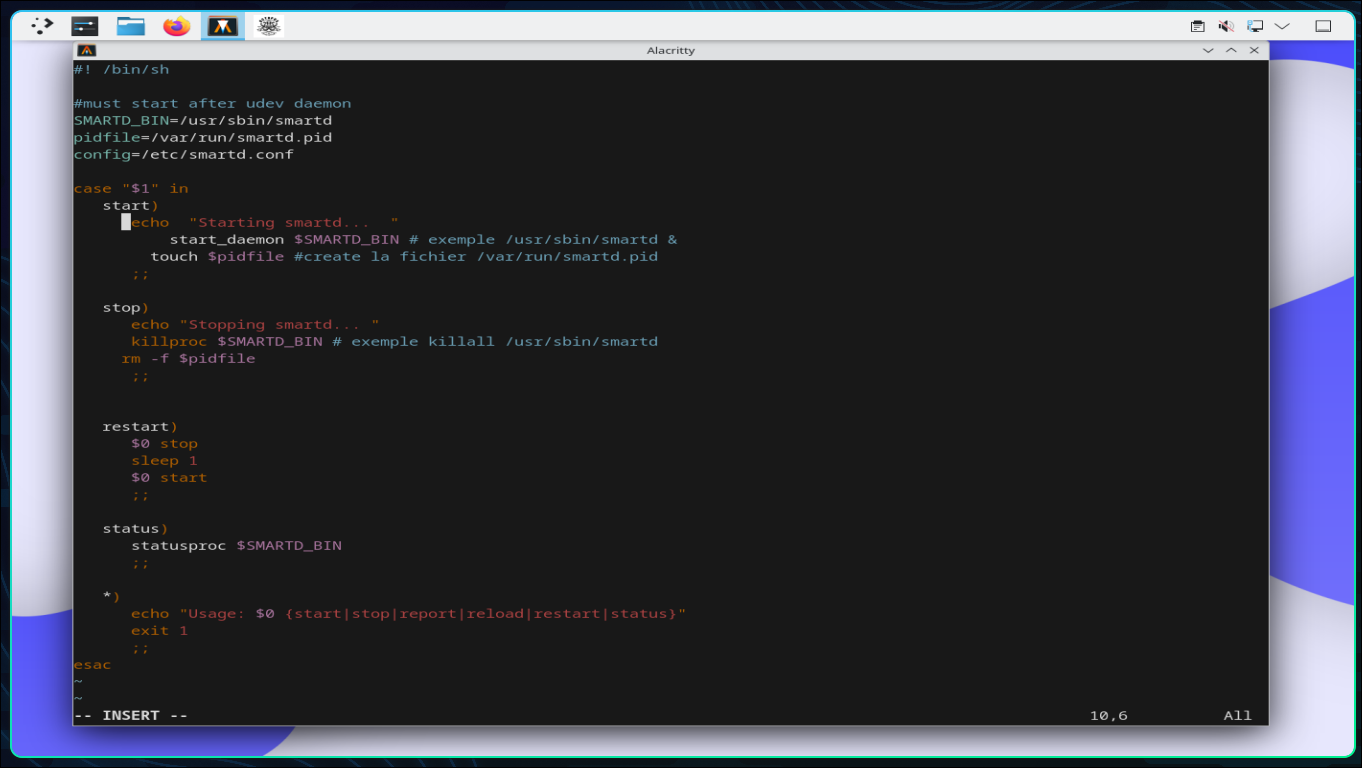
\includegraphics[width=0.85\textwidth]{images_pfe/smartdboots.png}
%  \caption{Script SystemV pour le démon smartd}
%  \label{fig:smartd_bootscript}
%\end{figure}

\section{Bibliothèques générales}
\label{subsec:general-lib}

Exemple  des bibliothèques utilitaires et de support :

\begin{table}[H]
    \centering
    \begin{tabular}{|c|p{8cm}|}
        \hline
        \textbf{Paquet}  & \textbf{Fonction principale} \\
        \hline
        dbus-glib & Liaison GLib pour D-Bus - Intégration des services de bus de messages dans les applications GLib \\
        \hline
        Fontconfig  & Configuration et personnalisation des polices système  \\
        \hline
        
        Wayland & Protocole de serveur d'affichage moderne (alternative à X11) pour la composition graphique \\
        \hline
        
    \end{tabular}
    \caption{Bibliothèques système et de support général}
    \label{tab:general-lib}
\end{table}




%\section{Bibliothèques graphiques et polices}
%\label{subsec:graphics-fonts}

%Paquets pour le rendu graphique et la gestion des polices :

%\begin{table}[H]
%    \centering
%    \begin{tabular}{|c|p{8cm}|}
%        \hline
%        \textbf{Paquet}  & \textbf{Fonction principale} \\
%        \hline
%        FreeType & Moteur de rendu de polices vectorielles \\
%        \hline
%        Fontconfig  & Configuration et personnalisation des polices système  \\
%        \hline
%        
%        Pixman  & Bibliothèque de manipulation de pixels bas niveau pour les opérations graphiques  \\
%        \hline
 %   \end{tabular}
 %   \caption{Bibliothèques graphiques et gestion des polices}
 %   \label{tab:graphics-fonts}
%\end{table}

%\textbf{Exemple d'installation du paquet harfBuzz-9.0.0} :  
%Le paquet HarfBuzz fournit un moteur de mise en forme de texte pour les polices OpenType.

%\textbf{Dépendances de harfBuzz} :
%\begin{verbatim}
%GLib-2.80.4       texlive-20240312   Graphite2-1.3.14   ICU-75.1
%FreeType-2.13.3 
%\end{verbatim}

%\textbf{Remarque} :  
%Ce paquet présente une \textbf{dépendance circulaire} avec FreeType-2.13.3 (bibliothèque de rendu de polices TrueType).  
%La procédure correcte est :  \\
%1. Compiler FreeType  \\
%2. Compiler HarfBuzz  \\
%3. Recompiler FreeType  \\

%\textbf{Exemple de compilation de harfbuzz depuis les sources} :
%\begin{verbatim}
%1: Résoudre toutes les dépendances listées ci-dessus
%2: Télécharger l'archive
%wget https://github.com/harfbuzz/harfbuzz/releases/download/9.0.0/harfbuzz-9.0.0.tar.xz
%3: Vérifier l'intégrité de l'archive
%   md5sum harfbuzz-9.0.0.tar.xz  # Doit être 0035c129cb1646ab1cff65e5ef7153db
%4: Extraire l'archive
%   tar -xvf harfbuzz-9.0.0.tar.xz
%5: Accéder au répertoire
%   cd harfbuzz-9.0.0
%6: Créer un répertoire de compilation
%   mkdir build && cd build
%7: Configurer (système de build : Meson avec Ninja)
%   meson setup ..             \
%      --prefix=/usr           \
%      --buildtype=release     \
%      -D graphite2=enabled 
%8: Compiler
%   ninja
%9: Tester
%   ninja test
%10: Installer
%   ninja install
%11: Nettoyer
%   rm -rf ../../harfbuzz-9.0.0
%\end{verbatim}

%\textbf{Programmes installés} :  
%hb-info, hb-ot-shape-closure, hb-shape, hb-subset, hb-view

%\textbf{Bibliothèques installées} :  
%\begin{itemize}
%  \item \texttt{libharfbuzz.so}
%  \item \texttt{libharfbuzz-cairo.so}
%  \item \texttt{libharfbuzz-gobject.so}
 % \item \texttt{libharfbuzz-icu.so}
 % \item \texttt{libharfbuzz-subset.so}
%\end{itemize}

%\textbf{Documentation} :  
%\texttt{/usr/share/gtk-doc/html/harfbuzz}
%\section{Paquets et bibliothèques réseau}
%\label{subsec:networking}

\section{Composants pour la connectivité et la gestion réseau} 

\begin{table}[H]
    \centering
    \begin{tabular}{|c|p{8cm}|}
        \hline
        \textbf{Paquet}  & \textbf{Fonction principale} \\
        \hline
        NetworkManager  & Gestion dynamique des connexions réseau (Wi-Fi, Ethernet, VPN)  \\
        \hline
       
        Net-tools  & Collection d'outils réseau  (\texttt{ifconfig}, \texttt{netstat}, \texttt{route}) \\
        \hline
    \end{tabular}
    \caption{Composants pour la connectivité et gestion réseau}
    \label{tab:network}
\end{table}



\section{Environnement graphique XORG}

\begin{figure}[H]
  \centering
  \begin{minipage}[b]{0.30\textwidth}
    
\includegraphics[width=\textwidth]{images_pfe/xorg.jpeg}
    \caption{Xorg}
  \end{minipage}\hfill
  \begin{minipage}[b]{0.30\textwidth}
    
\includegraphics[width=\textwidth]{images_pfe/wayland.png}
    \caption{Wayland}
  \end{minipage}
  \caption{Xorg et Wayland}
  \label{fig:xorgwayland}
\end{figure}
\FloatBarrier

Il existe des environnements graphiques sous GNU/Linux :

\begin{itemize}
    \item \textbf{Xorg} : ancien, basé sur une architecture \textbf{client-serveur}.
    \item \textbf{Wayland} : a émergé comme une alternative moderne à Xorg. Il prend en charge de nombreuses animations et personnalisations. Cependant, il dépend fortement des capacités 3D du GPU, ce qui peut entraîner des bugs lorsqu’il est utilisé dans une machine virtuelle.
\end{itemize}

C’est pourquoi nous avons choisi d’implémenter \texttt{Xorg} par défaut dans notre distribution, afin de garantir une \textbf{compatibilité maximale} avec tous les environnements.

\subsection*{Exemples d'applications et bibliothèques Xorg}

\begin{table}[H]
    \centering
    \begin{tabular}{|c|p{8cm}|}
        \hline
        \textbf{Paquet}  & \textbf{Fonction principale} \\
        \hline
        xterm & Émulateur de terminal standard pour Xorg \\
        \hline
        xinit  & Utilitaire de lancement du serveur X et session utilisateur \\
        \hline
        libX11  & Bibliothèque cliente principale X11 (gestion fenêtres/événements) \\
        \hline
        xcursor-themes & Collection d'icônes de curseur pour X11 (thèmes par défaut) \\
        \hline
    \end{tabular}
    \caption{Applications et utilitaires d'entrée Xorg}
    \label{tab:xorg-apps}
\end{table}

\textcolor{blue}{Pour plus d’informations sur Xorg, voir \cite{doc_xorg}.}\\
\textcolor{blue}{Pour plus d’informations sur les bibliothèques Xorg, voir \cite{bibliotheques_xorg}.}

\section{Environnement de bureau}
\label{subsec:desktop-env}


Un environnement de bureau offre une interface plus complète au système d’exploitation, avec un ensemble d’utilitaires et d’applications intégrés.

\textbf{KDE} est un environnement de bureau complet, reposant sur le framework \textbf{Qt}, rassemblant de nombreuses applications et une vaste communauté d’utilisateurs.\\
 KDE  se divise en deux blocs principaux :  
\begin{itemize}
  \item \textbf{KDE Frameworks 6} (KF6)   et \textbf{KDE Plasma 6} 
  
\end{itemize}



\subsection{KDE Frameworks 6}
\label{sssec:kf6}

KDE Frameworks 6 est un ensemble de bibliothèques basées sur Qt 6 et QML

Exemple des  bibliothèques


% KDE Frameworks 6
\begin{table}[H]
    \centering
    \begin{tabular}{|c|p{8cm}|}
        \hline
        \textbf{Paquet}  & \textbf{Fonction principale} \\
        \hline
       
        extra-cmake-modules  & Modules CMake supplémentaires pour la construction des logiciels KDE \\
        \hline
        kapidox  & Outil de génération de documentation API pour les frameworks KDE \\
        \hline
        
    \end{tabular}
    \caption{Composants clés de KDE Frameworks 6}\\
    \label{tab:kf6}
\end{table}

\textcolor{blue}{Pour plusieur information sur kde framework  \cite{framework_kde}}.\\

\subsection{Applications KDE}
\label{sssec:kde-apps}

Pour enrichir l’expérience utilisateur, nous installons plusieurs applications KDE ,Exemple :

\begin{table}[H]
    \centering
    \begin{tabular}{|c|p{8cm}|}
        \hline
        \textbf{Paquet} & \textbf{Fonction principale} \\
        \hline
        konsole  & Terminal émulateur avancé avec onglets et profils personnalisables \\
        \hline
        dolphin & Gestionnaire de fichiers phare de KDE avec navigation par onglets \\
        \hline
        plasma-activities  & Gestion des espaces de travail virtuels et suivi des tâches \\
        \hline
        khelpcenter  & Centre d'aide unifié pour la documentation KDE et manuels \\
        \hline
    \end{tabular}
    \caption{Applications principales de l'écosystème KDE}
    \label{tab:kde-apps}
\end{table}

\subsection{KDE Plasma 6}
\label{sssec:plasma6}

KDE Plasma est un ensemble de paquets construits sur KDE Frameworks et QML, constituant l’environnement d’affichage Plasma.

Exemple des Composants Plasma 6


\begin{table}[H]
    \centering
    \begin{tabular}{|c|p{8cm}|}
        \hline
        \textbf{Paquet}  & \textbf{Fonction principale} \\
        \hline
        kscreenlocker  & Système de verrouillage d'écran sécurisé avec intégration PAM \\
        \hline
        plasma-desktop  & Environnement de bureau principal avec panneau et widgets \\
        \hline
        plasma-workspace  & Couche d'intégration pour la gestion des sessions Plasma \\
        \hline
        breeze  & Thème visuel par défaut de Plasma (icônes, décorations de fenêtre) \\
        \hline
    \end{tabular}
    \caption{Composants fondamentaux de KDE Plasma 6}
    \label{tab:plasma6}
\end{table}

\textcolor{blue}{Pour plusieur information sur kde Plasma   \cite{environnement_plasma}}.\\
\section{Thème KDE Plasma et sélecteur de domaine}
\label{sssec:kde-theme-domain}

Nous avons choisi de personnaliser le thème KDE Plasma pour qu’il reflète l’identité de \textsc{Kraken OS}.  
Cette personnalisation inclut :
\begin{itemize}
  \item la modification du panneau par défaut (couleurs, transparences) ;
  \item l’installation de \texttt{cairo‑dock} pour un lanceur plus ergonomique ;
  \item la création d’environnements visuels distincts pour chaque domaine scientifique (web, mobile, IA/ML, cybersécurité, mathématiques, physique, etc.).
\end{itemize}

Nous avons également développé une application \textbf{simple}, reposant sur les activités KDE Plasma, permettant à l’utilisateur de basculer d’un domaine à l’autre.\\

\begin{figure}[H]
  \centering
  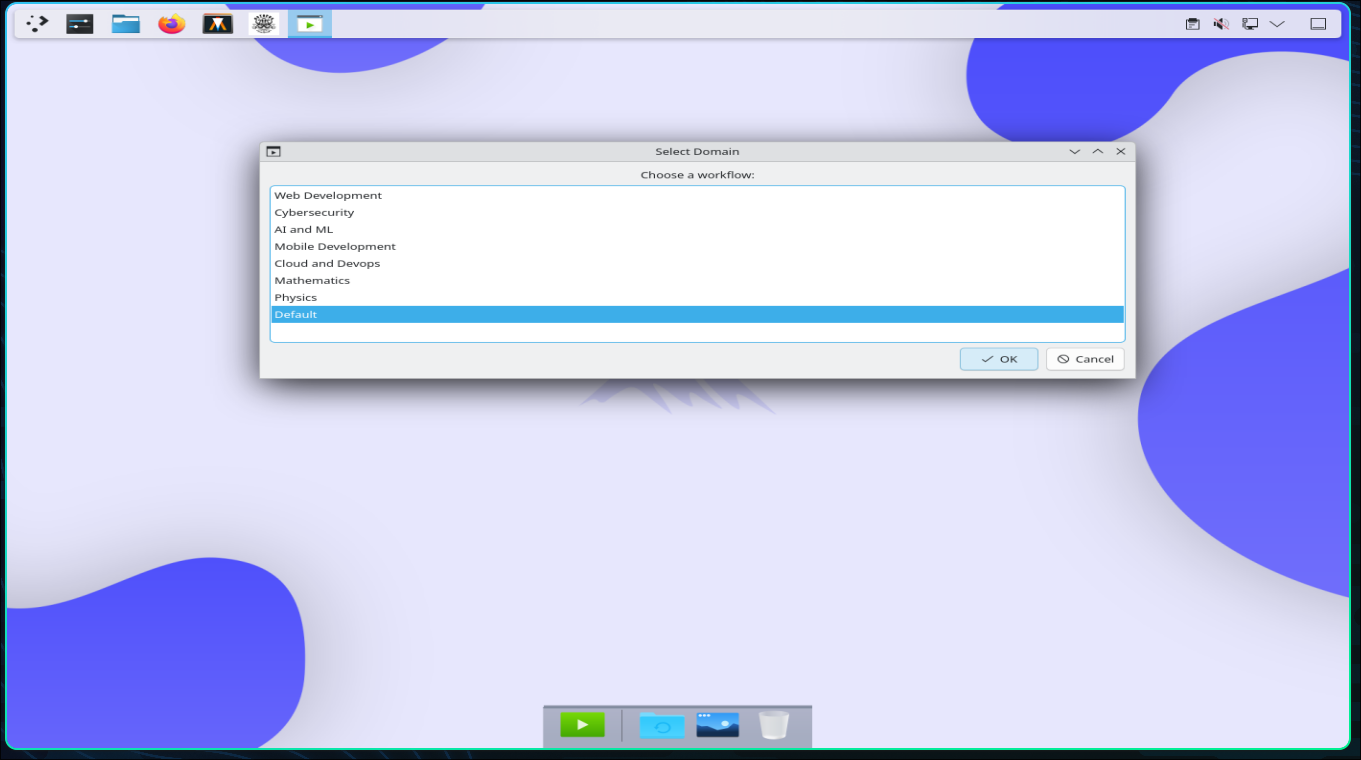
\includegraphics[width=1\textwidth]{images_pfe/defaultswitcher.png}
  \caption{Sélecteur de domaine par défaut de \textsc{Kraken}}
  \label{fig:dks}
\end{figure}

\textcolor{blue}{Pour voir une vidéo de prévisualisation de notre environnement KDE Plasma personnalisé, voir \cite{kde_preview}.}\\

\textcolor{blue}{Le code source de l’application qui permet de changer de domaine est disponible dans \cite{switch_domaine}.}\\
\textcolor{blue}{Pour voir une vidéo de prévisualisation de notre application de changement de domaine, voir \cite{kraken_doamin_switcher}.}\\





 \clearpage

\section{Navigateur web}
\label{subsec:web-browser}

Nous avons choisi d’installer le navigateur \textbf{Firefox}, en raison de sa philosophie open source et de sa simplicité.  
Le navigateur Brave, quant à lui, est un paquet volumineux nécessitant environ 30 Go de données pour sa compilation, car il dépend de Chromium.  
%List des depandances de firefox  :
%\begin{verbatim}
%Cbindgen-0.27.0       GTK+-3.24.43          libnotify-0.8.3   LLVM-18.1.7             
%nodejs-20.16.0        PulseAudio-17.0       Python-3.12.5     startup-notification-0.12
%UnZip-6.0             alsa-lib-1.2.12       SQLite-3.46.1     NASM-2.16.03    
%cURL-8.9.1            Doxygen-1.12.0        FFmpeg-7.0.2      GeoClue-2.7.1            
%liboauth-1.0.3        pciutils-3.13.0       Valgrind-3.23.0    Wget-1.24.5              
%Wireless-Tools-29     yasm-1.3.0            nss-3.103            
%\end{verbatim}
\begin{figure}[H]
  \centering
  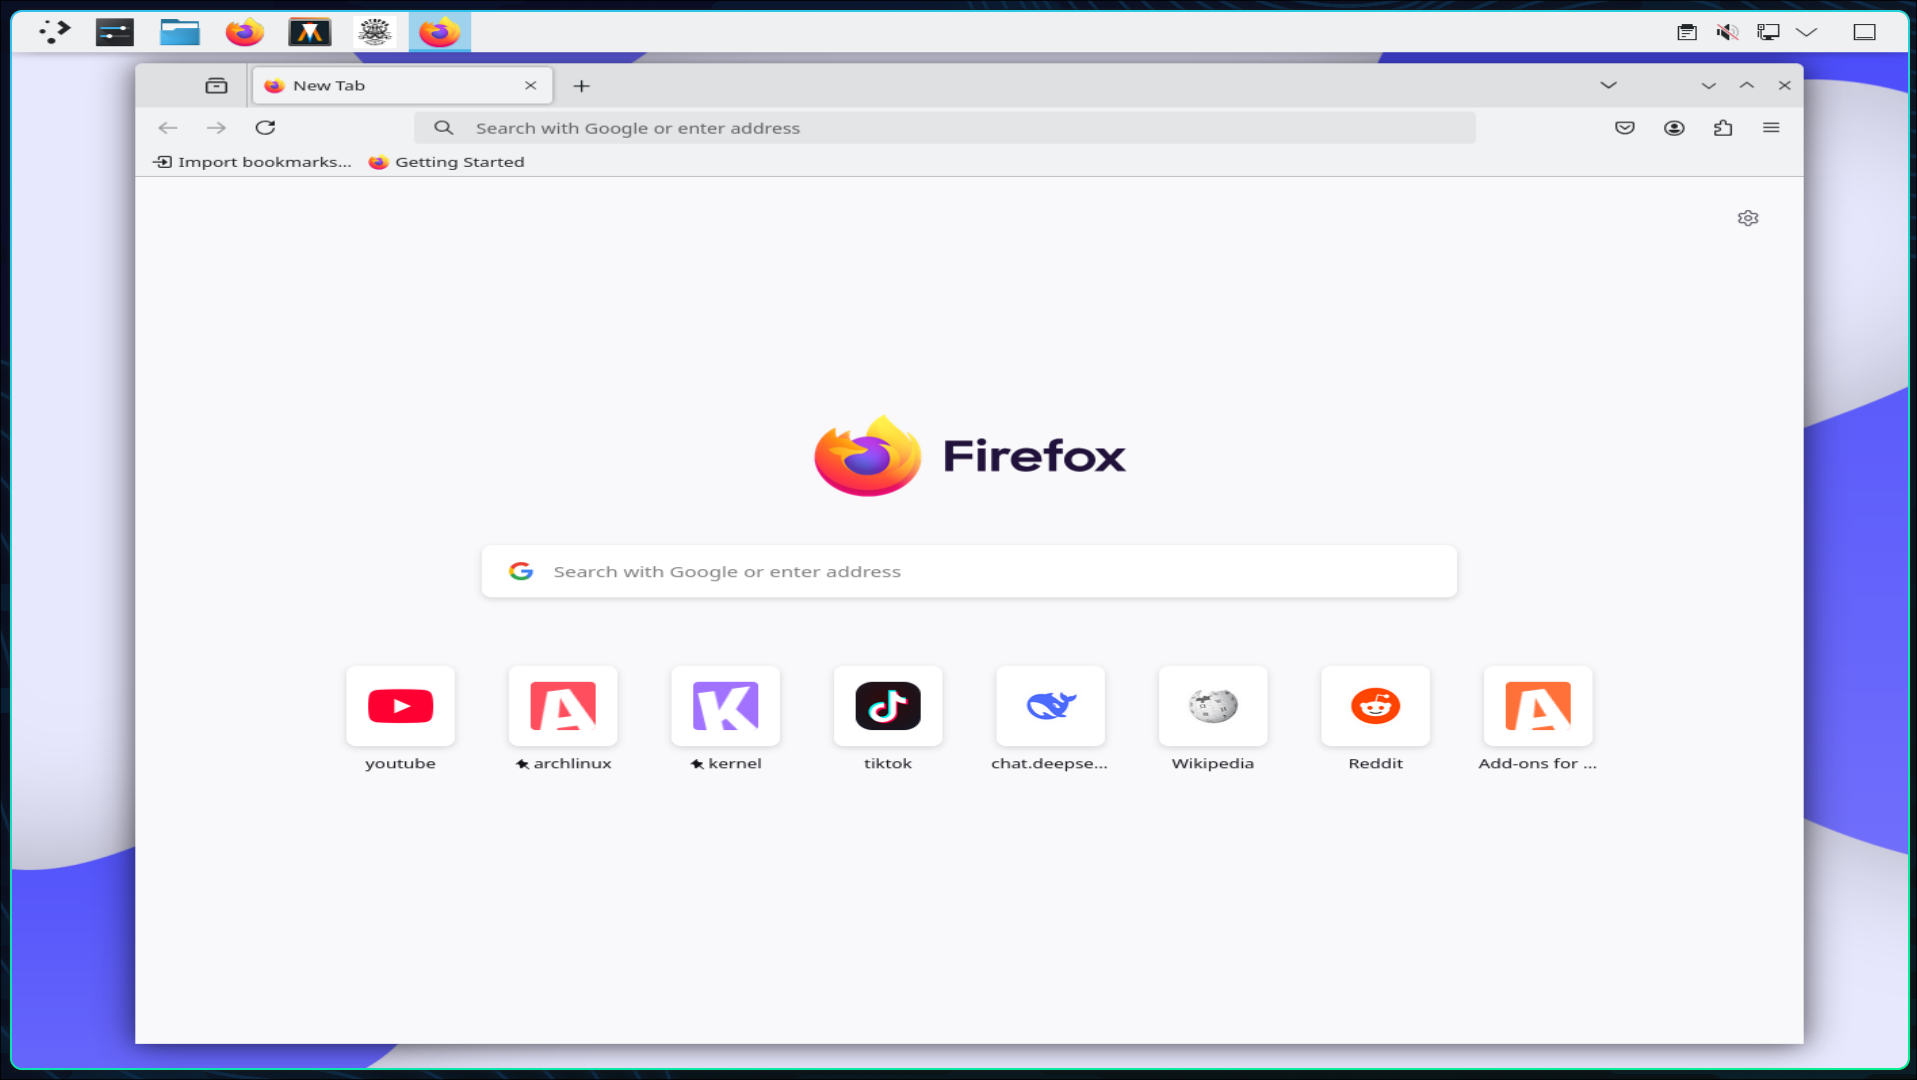
\includegraphics[width=1\textwidth]{images_pfe/firefox.png}
  \caption{Navigateur web firefox}
  \label{fig:firefox-custom}
\end{figure}



 
\section{Gestionnaire d’affichage et thème du bootloader GRUB}
\label{subsec:sddm-theme}

\subsection{Thème SDDM}
Un gestionnaire d'affichage (login manager) est une interface graphique lancée au démarrage du système, remplaçant le shell par défaut. 

Pour sa légèreté et sa facilité de personnalisation, nous avons retenu \textbf{SDDM} comme gestionnaire d’affichage.  
Basé sur Qt/QML, il permet une création intuitive de thèmes visuels grâce à son langage déclaratif.

\begin{figure}[H]
  \centering
  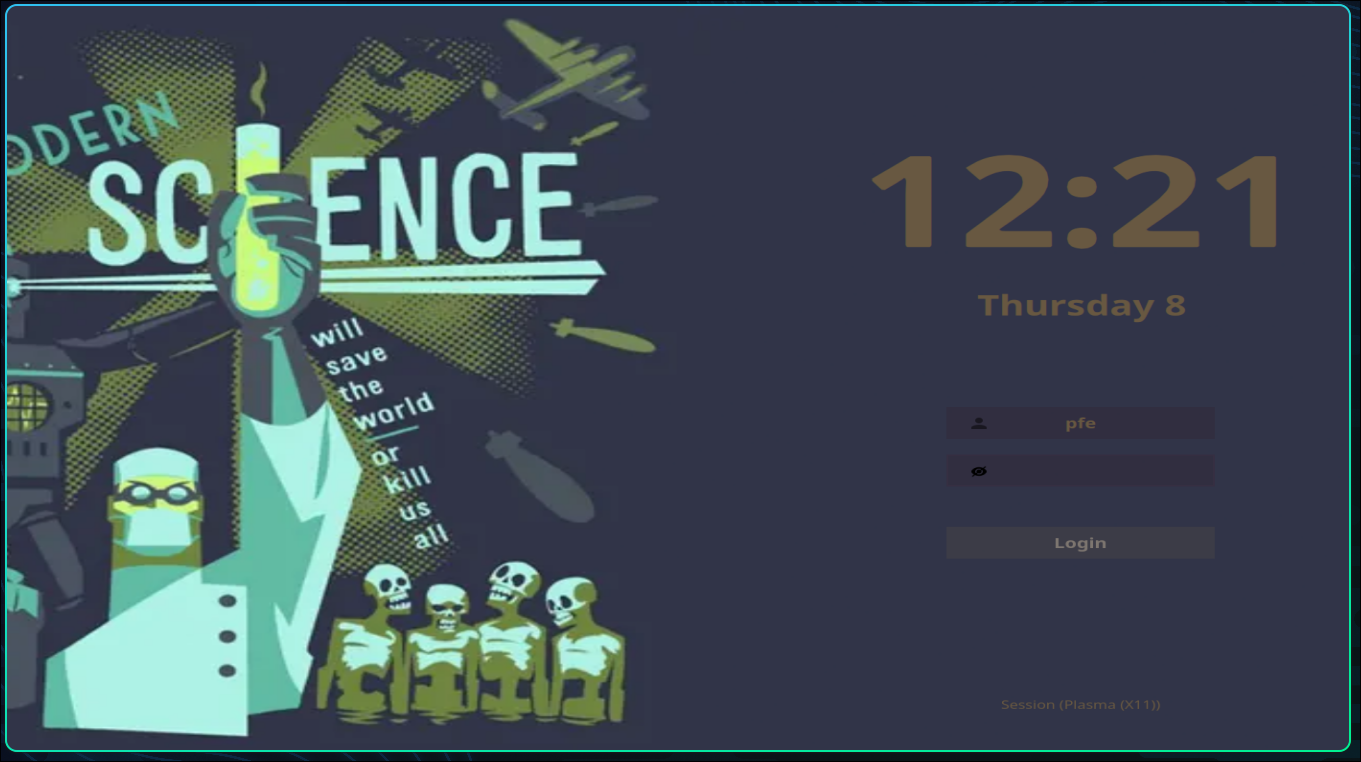
\includegraphics[width=1\textwidth]{images_pfe/sddmkrakentheme.png}
  \caption{Thème SDDM personnalisé pour \textsc{Kraken OS}}
  \label{fig:sddm-custom}
\end{figure}

    \textbf{Remarque} : Ce thème, nommé SDDM-Astronaut, est principalement développé par Keyitdev.
Étant donné que le thème est sous licence GPL, nous pouvons le modifier. Nous avons donc apporté des modifications simples\\

\textcolor{blue}{Version originale du thème Astronaut : disponible dans \cite{sddm_theme_astronaut}}.\\
\textcolor{blue}{Notre Version modifiée : disponible dans \cite{sddm_theme_kraken}}.\\
\subsection{Thème GRUB}
\label{subsec:grub-theme}

Le thème GRUB a été adapté à la charte graphique de la distribution. Sa structure minimale comprend :
\begin{itemize}
    \item Un fichier principal \texttt{theme.txt} 
    \item Configuration des polices, couleurs et résolution
   
\end{itemize}



\begin{figure}[H]
  \centering
  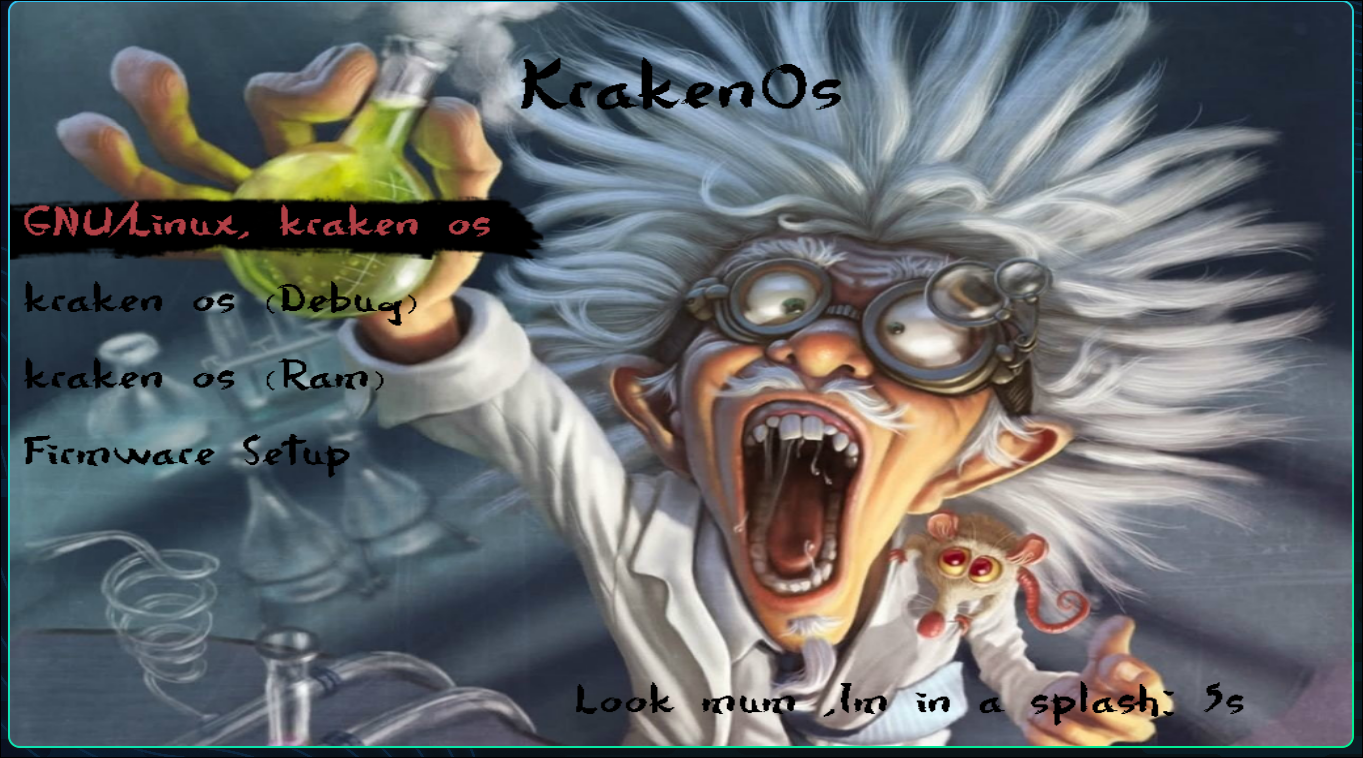
\includegraphics[width=1\textwidth]{images_pfe/grubthemekraken.png}
  \caption{Thème GRUB personnalisé pour \textsc{Kraken OS}}
  \label{fig:grub-custom}
\end{figure}

\textcolor{blue}{Code source disponible dans \cite{theme_grub}}.
\section{Conclusion}
À ce stade, nous disposons d'une distribution Linux fonctionnelle et enrichie. Cependant, il manque encore un composant essentiel : un \textbf{gestionnaire de paquets} permettant aux utilisateurs d'installer, mettre à jour ou supprimer des logiciels de manière cohérente.

Dans le prochain chapitre, nous aborderons le développement et l'intégration de notre gestionnaire de paquets 